\chapter{Introduction} \label{chap:intr}
%
%
\acrfull{ai} is a young and promising field in science and engineering which started to be investigated after World War II \cite{russell_artificial_2009}. \acrshort{ai} is an 'umbrella term' that includes multiples approaches and that envelops a large diversity of domains such as computer vision, natural language processing, voice recognition, etc.
\acrfull{ml}, one of \acrshort{ai} subfield founded in the 1950s, has revolutionized several technology realms in the last decades \cite{alom_history_2018}. \textcite{mitchell_machine_1997} gives us a definition of what \acrshort{ml} is: "\textit{The concept of \acrshort{ml} relates to the question of how to construct computer programs that automatically improve with experience}" (that can learn).

\textcite{arnold_introduction_2011} reported that statistical machine learning is concerned with the selection of the most relevant features from the inputs to solve a specific problem. A promising solution would be automatic learning of the features using \acrfull{nn}. From this idea spawned \acrfull{dl} architectures, composed of layers of non-linearity processing. Since the last decades, \acrshort{dl} is gaining in interest and the domains of applications have grown rapidly \cite{wason_deep_2018}. The accuracy of those models has also increased. For example, in 2015, the image classification model on ImageNet dataset achieved 94.6\% of accuracy on average \cite{russakovsky_imagenet_2015}.

A type of \acrshort{dl} model, \acrfull{cnn}, has demonstrated its effectiveness in image classification object detection, and speech recognition \cite{shawahna_fpga-based_2019}. However, the accuracy of such models comes at the price for a large computational cost (billions of operations and millions of parameters) \cite{szegedy_going_2014}. To train and evaluate a large-scale \acrshort{cnn}, general \acrfull{cpu} would not provide enough computational power \cite{liu_fpga-based_2019}. To improve the throughput and latency of the \acrshort{cnn}, dedicated hardware such as \acrfull{gpu}, \acrfull{asic} and \acrfull{fpga} can be used. The dominant platforms to perform \acrshort{cnn} inferences are \acrshort{cpu} and \acrshort{gpu} clusters because they offer the best performance in terms of computational throughput but those are power-hungry \cite{liu_uniform_2019}.
\acrshort{fpga} and \acrshort{asic} seem then to be a promising solution because they are more energy-efficient. This has been demonstrated by \textcite{qasaimeh_comparing_2019}, where FPGA outperforms \acrshort{gpu} as the vision application’s pipeline complexity grows (which is the case for \acrshort{cnn}). We can observe in table \ref{tab:benchener} the FPGA’s energy reduction ratios to GPU for various vision application’s pipeline. Moreover, an \acrshort{fpga}-based \acrshort{cnn} accelerator is more suitable than an \acrshort{asic} because it is more time and cost-effective when designing and verifying a process \cite{motamedi_placid_2017}.
%
\begin{table}
    \center
    \begin{tabular}{|c|c|}
        \hline
        Pipeline & Energy/frame (mJ/f) \\
        \hline
        Background Subtraction & 1.74 $\times$\\
        \hline
        Color Segmentation & 1.86 $\times$ \\
        \hline
        Harris Corners Tracking & 3.94 $\times$ \\
        \hline
        Stereo Block Matching & 8.83 $\times$ \\
        \hline
    \end{tabular}
    \caption{FPGA’s Reduction Ratios with respect to GPU \cite{qasaimeh_comparing_2019}}
    \label{tab:benchener}
\end{table}

Still, \acrshort{gpu} is currently the most dominant platform to accelerate \acrshort{cnn}, trends confirm that \acrshort{fpga} will be more suitable to accelerate \acrshort{cnn}. Two reasons can explain that: first, the advance in \acrshort{fpga} technology shows that the performance disparity between \acrshort{fpga} and \acrshort{gpu} has lessened; second, recent trends in \acrshort{cnn} utilize sparsity and extreme compact data types which is in the favor of the \acrshort{fpga}s, because they are designed to handle irregular parallelism and custom data type \cite{nurvitadhi_can_2017}. However, \acrshort{fpga} is resource-constraint (limited memory, I/O bandwidth, and computing resources) and the challenge is to find a mapping between the computational model and the execution model.

\acrshort{cnn} consists of two phases: a training stage where the model learns (back-propagation algorithm \cite{lecun_backpropagation_1989}) and the inference stage where the model makes a prediction on new data samples (feed-forward algorithm \cite{zhang_optimizing_2015}). We can see the process in figure \ref{fig:traininf}. Usually, \acrshort{cnn}s are trained once using \acrshort{gpu} or \acrshort{fpga} and inference is executed every time the \acrshort{cnn} has a new input to process. Most efforts have then been focused on accelerating the inference stage. The core of this work is therefore aimed at proposing a way to accelerate the inference of a model through weights pruning. It is not efficiently usable on a \acrshort{gpu} because of the irregular data access and the custom data type of the non-pruned weights.
%
\begin{figure}
    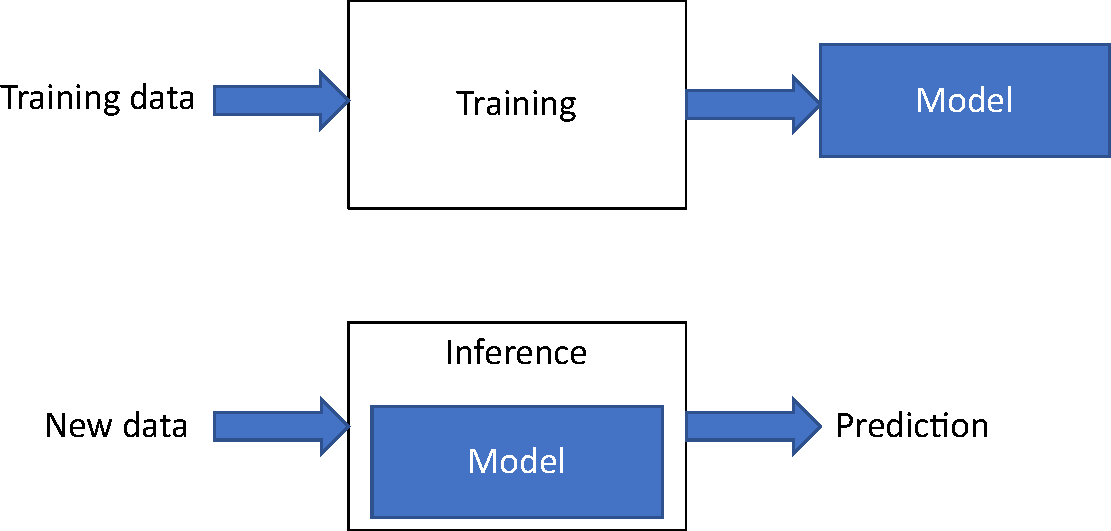
\includegraphics[width=\textwidth]{traininf.pdf}
    \caption{\acrshort{cnn} setup for predicting new data}
    \label{fig:traininf}
\end{figure}

\noindent This work concentrates on building an architecture using pruning on depthwise separable convolution, an alternative way to perform convolution which uses fewer parameters and has a lesser computational complexity. The objective of this work is then to build an efficient architecture on \acrshort{fpga} implementing a sparse \acrshort{cnn} network using depthwise separable convolution. To show the achievability, we have chosen MobileNetV2 because it offers state-of-the-art performance.
%
%
\section*{Structure of the thesis}
%
%
This master thesis is composed of 8 chapters.

Chapter \ref{chap:cnn} details the theory behind \acrshort{cnn} and goes deeper into its computational background. It develops also model compression optimizations allowing a reduction of the size and the computational complexity of the model.

The concept of \acrshort{fpga} is explained in chapter \ref{chap:fpga}. We detail there the workflow and \acrshort{fpga} designs. Solutions to the issues of mapping a \acrshort{cnn} model on \acrshort{fpga} are described too.

Chapter \ref{chap:inf} discusses the state-of-art \acrshort{fpga} inference optimization techniques. We do a review of the different approaches and see which are the more promising ones.

As we have shown in chapter \ref{chap:inf} why we have chosen pruning to be the core of this work, chapter \ref{chap:compress} develops state-of-the-art architecture using pruning to accelerate inference.

Chapter \ref{chap:arch} is focused on how to build an efficient architecture on \acrshort{fpga} and uses this knowledge to design our architecture using pruning and depthwise separable convolution.

Chapter \ref{chap:measure} explains the simulation on SystemVerilog of the architecture developed in chapter \ref{chap:arch} and details the experiments on this simulation. Potential improvements will be discussed.

Finally, a conclusion on results obtained and discussion on future works is done in chapter \ref{chap:ccl}.

\afterpage{\blankpage}
\cleardoublepage
\newpage
